\begin{Example}[toxaemia]{Toxaemic symptoms in pregnancy}
\citet{Brown-etal:83} gave the data in \tabref{tab:toxtab}
on the occurrence of signs of toxaemia (hypertension and protein urea)
among 13,384 expectant mothers in Bradford, England in their first pregnancy.
The mothers are classified by social class, and by the
number of cigarettes smoked per day.
There are thus two response variables, and two explanatory variables
in this $2 \times 2 \times 5 \times 3$ table.
\begin{table}[htb]
 \caption{Toxaemic symptoms of mothers during pregnancy. From: }\label{tab:toxtab}
 \begin{center}
 \begin{tabular}{c| rrrr| rrrr| rrrr}
  \hline
\multicolumn{1}{r|}{Smoking}
    & \multicolumn{4}{c|}{0} & \multicolumn{4}{c|}{1-19} & \multicolumn{4}{c}{20+} \\

\multicolumn{1}{r|}{Hypertension}
    & \multicolumn{2}{c}{Yes} & \multicolumn{2}{c|}{No} & \multicolumn{2}{c}{Yes} & \multicolumn{2}{c|}{No}  & \multicolumn{2}{c}{Yes} & \multicolumn{2}{c}{No} \\
\multicolumn{1}{r|}{Protein urea}
    & Yes & No & Yes & No & Yes & No & Yes & No & Yes & No & Yes & No \\ 
  \hline
Social Class \\
  \hline
  1 &  28 &   82 &  21 &  286 &   5 &  24 &   5 &   71 &  1 &  3 &  0 & 13 \\ 
  2 &  50 &  266 &  34 &  785 &  13 &  92 &  17 &  284 &  0 & 15 &  3 & 34 \\ 
  3 & 278 & 1101 & 164 & 3160 & 120 & 492 & 142 & 2300 & 16 & 92 & 32 & 383 \\ 
  4 &  63 &  213 &  52 &  656 &  35 & 129 &  46 &  649 &  7 & 40 & 12 & 163 \\ 
  5 &  20 &   78 &  23 &  245 &  22 &  74 &  34 &  321 &  7 & 14 &  4 & 65 \\ 
  \hline
 \end{tabular}
 \end{center}
\end{table}


The questions of main interest are how the occurrence of each symptom
varies with class and smoking, and how the association between them
varies. It is useful, however, to examine first the marginal relationship between
the two responses, and between the two predictors.
These are produced with the \macro{mosaic} as shown below.
The parameter \pname{PLOTS=2} gives a plot of the first two variables,
according to the order in which the data are sorted.
Re-sorting to make \pname{hyper} and \pname{urea} vary most rapidly
gives the second plot.  Both plots are shown in \figref{fig:tox41}.
\begin{listing}
%include catdata(toxaemia);

data toxaemia;
   set toxaemia;
   sm = put(smoke, smoke.);

%mosaic(data=toxaemia, var=Class Sm Hyper Urea, plots=2, htext=2,
   title=%str(Predictors: Class, Smoke));

proc sort data=toxaemia;
   by class sm descending urea descending hyper;
%mosaic(data=toxaemia, var= Hyper Urea Sm Class, plots=2, sort=no, htext=2,
   title=%str(Hypertension and Protein Urea));
\end{listing}

%% one figure
\begin{figure}[htb]
  \centering
  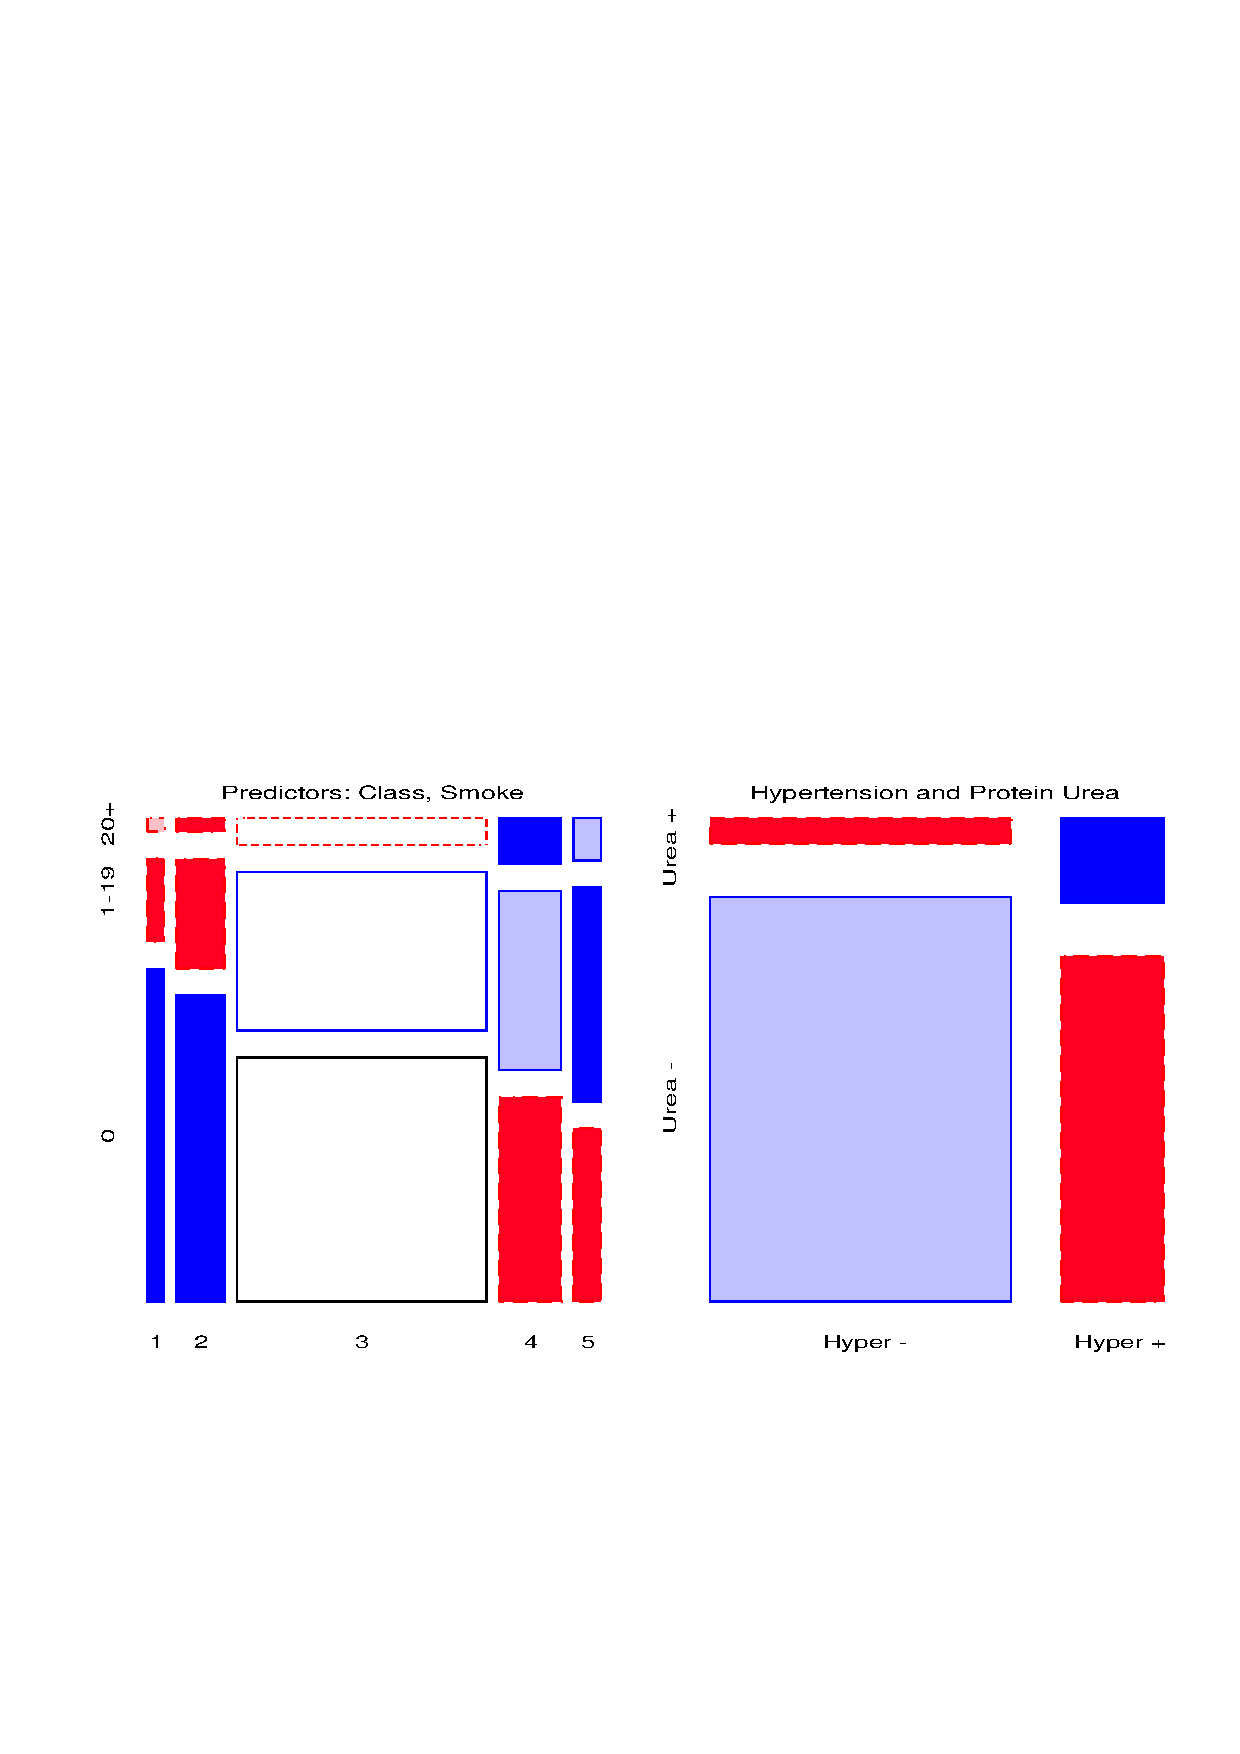
\includegraphics[scale=.6,clip]{tox41}
  \caption{Mosaic displays for toxaemia data: Predictor and Response associations}%
  \label{fig:tox41}
\end{figure}
We see in \figref{fig:tox41} that the majority of the mothers are in the
third social class, and that smoking is negatively related to social
class, with the highest levels of smoking in classes 4 and 5.
Within the responses, the great majority of women exhibit neither symptom,
but showing one symptom makes it more likely to show the other.
Marginally, hypertension is somewhat more prevalent than protein urea.

We next examine how the association between responses varies with
social class and with smoking.
\figref{fig:tox42}  shows a collection of partial
mosaic plots of the association between hypertension and urea,
for each level of smoking, collapsed over social class.
\figref{fig:tox43} is similar, but stratified by social class.
These statements produce \figref{fig:tox42}:
\begin{listing}
proc freq data=toxaemia order=data;
   tables hyper * urea * smoke / out=sum1;
   weight count;
%mosaic(data=sum1,  var= Hyper Urea Smoke, sort=no, by=Smoke, htext=3);
\end{listing}

Ignoring social class, the association between hypertension and protein urea
decreases with smoking.
Ignoring smoking, the association is greatest in social class 3.
However, these two symptoms are positively associated in all cases.

%% one figure
\begin{figure}[htb]
  \centering
  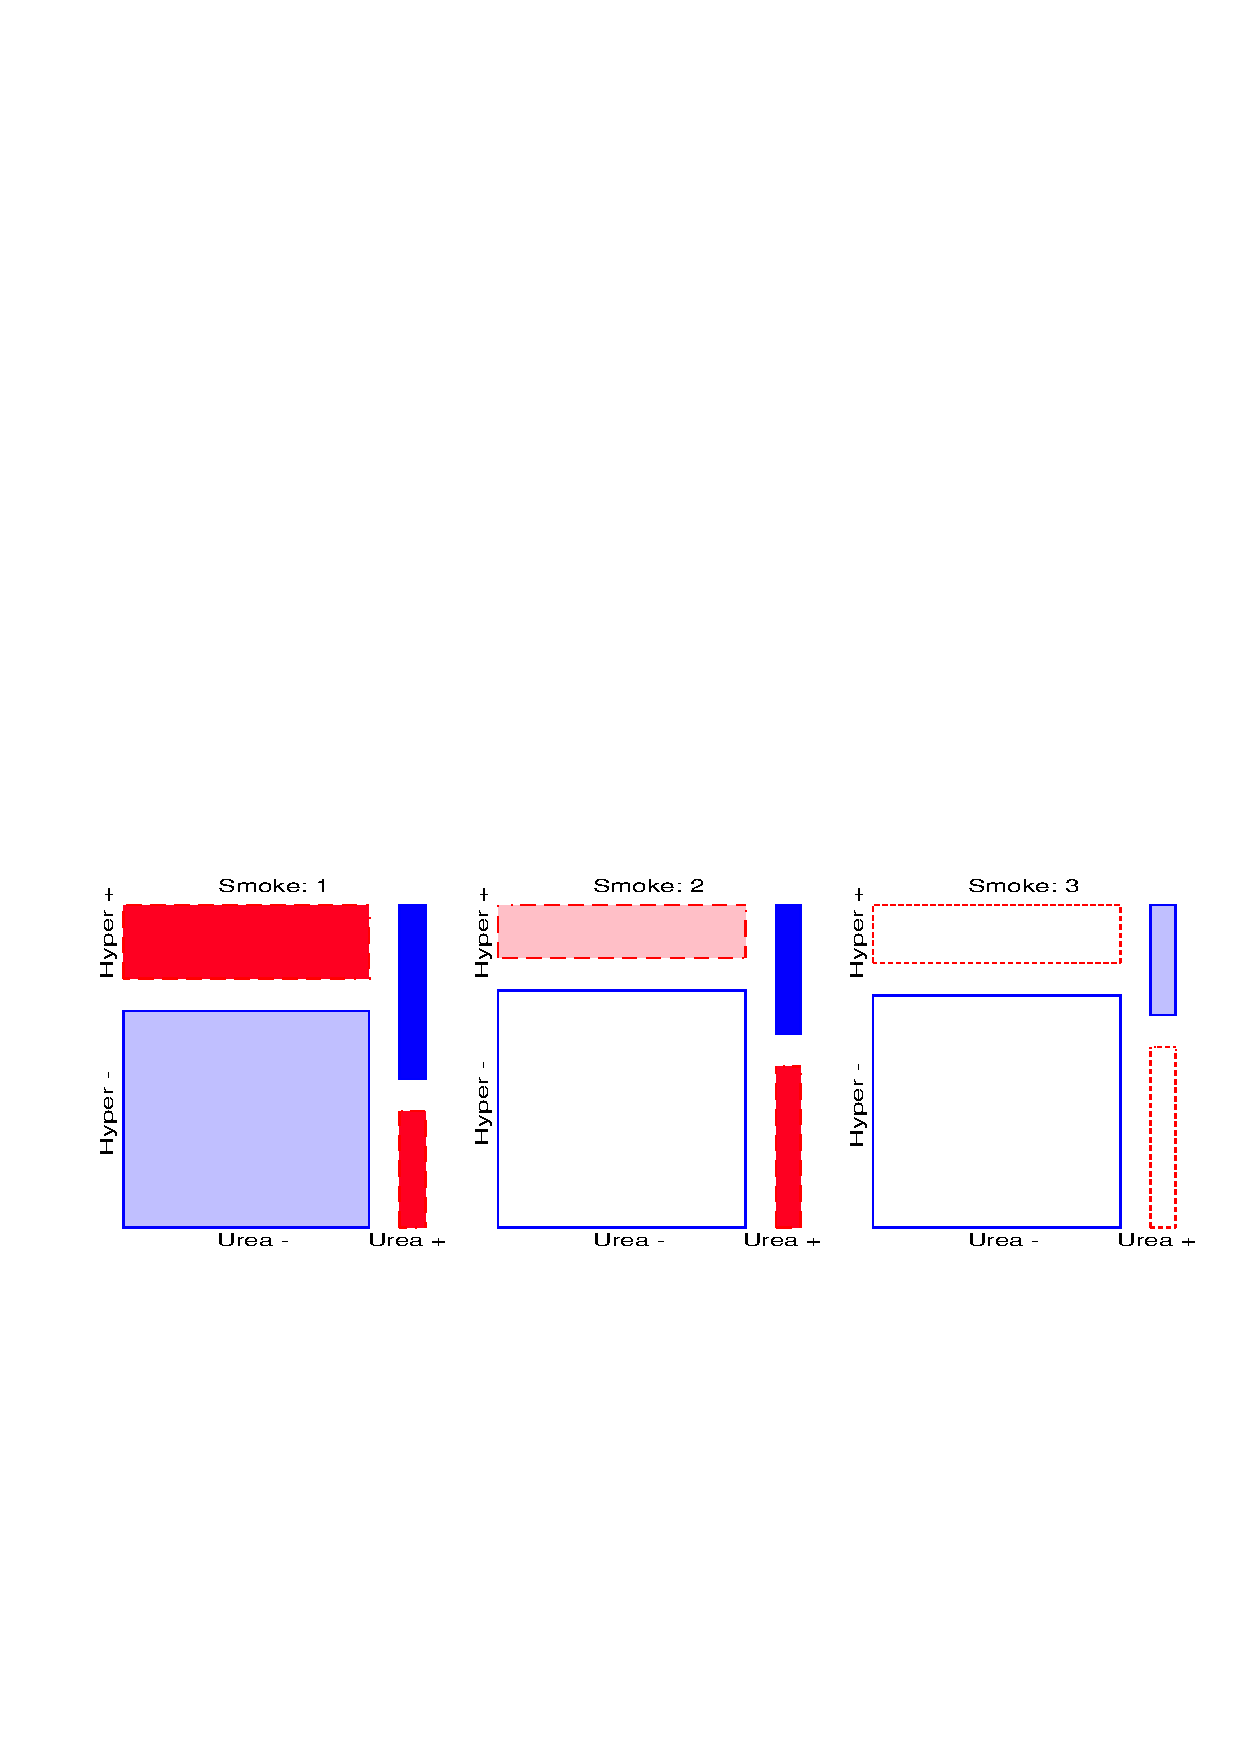
\includegraphics[scale=.75,clip]{tox42}
  \caption{Toxaemia data: Response associations by Smoking}%
  \label{fig:tox42}
\end{figure}
%% one figure
\begin{figure}[htb]
  \centering
  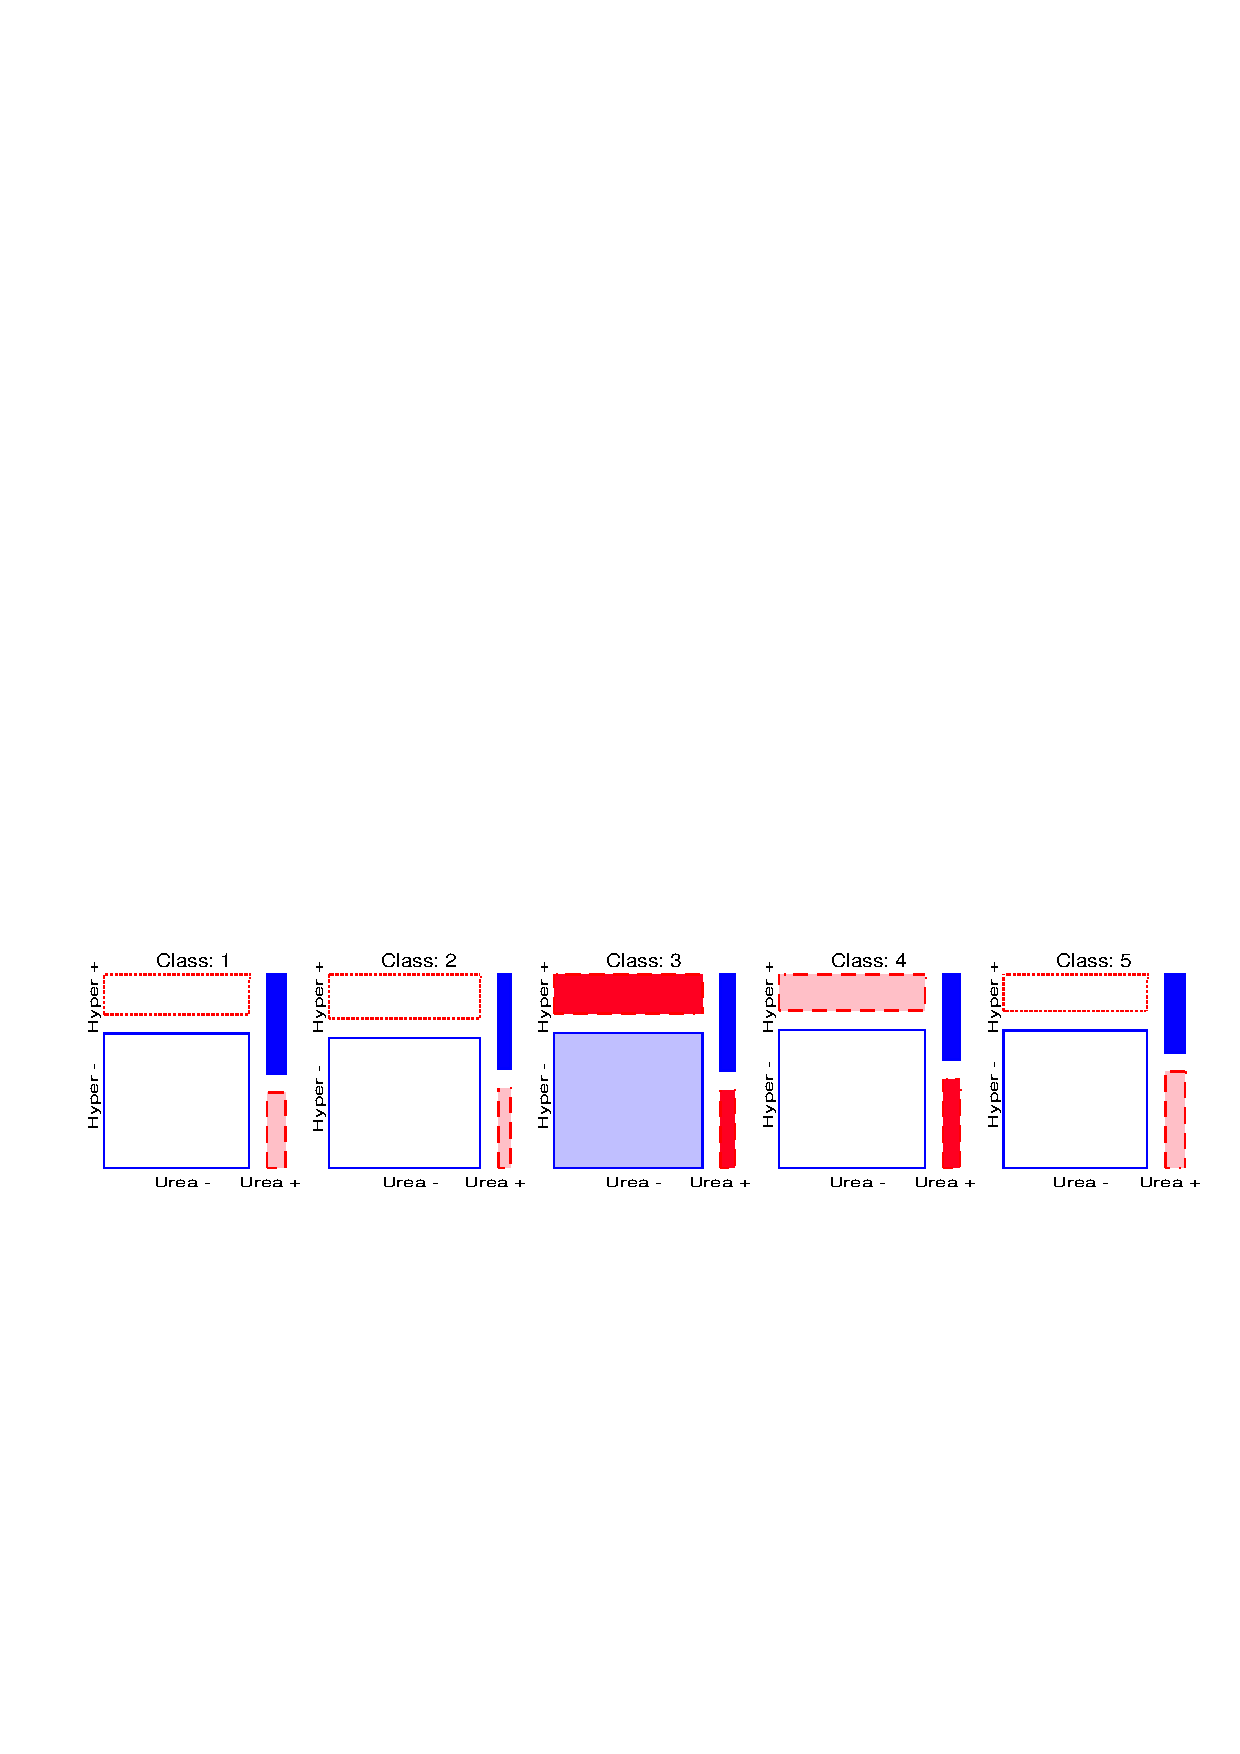
\includegraphics[scale=.75,clip]{tox43}
  \caption{Toxaemia data: Response associations by Social Class}%
  \label{fig:tox43}
\end{figure}

Our initial overview of the data is completed
by calculating and plotting the empirical logit for each
symptom and the log odds ratio, within each class-smoke population.
This is done in the same way as in \exref{ex:ashford},
except that there are now two explanatory factors.  Consequently,
it is most useful to make separate plots for each of the logits
and the log odds ratio,
each plot shows the response measure against class, with
separated curves for the levels of smoking.
The logits for hypertension and for protein urea are shown in \figref{fig:tox11}; the log odds ratio is shown in \figref{fig:tox13}.

%% two subfig side-by-side
\begin{figure}[htb]
 \begin{minipage}[t]{.49\linewidth}
  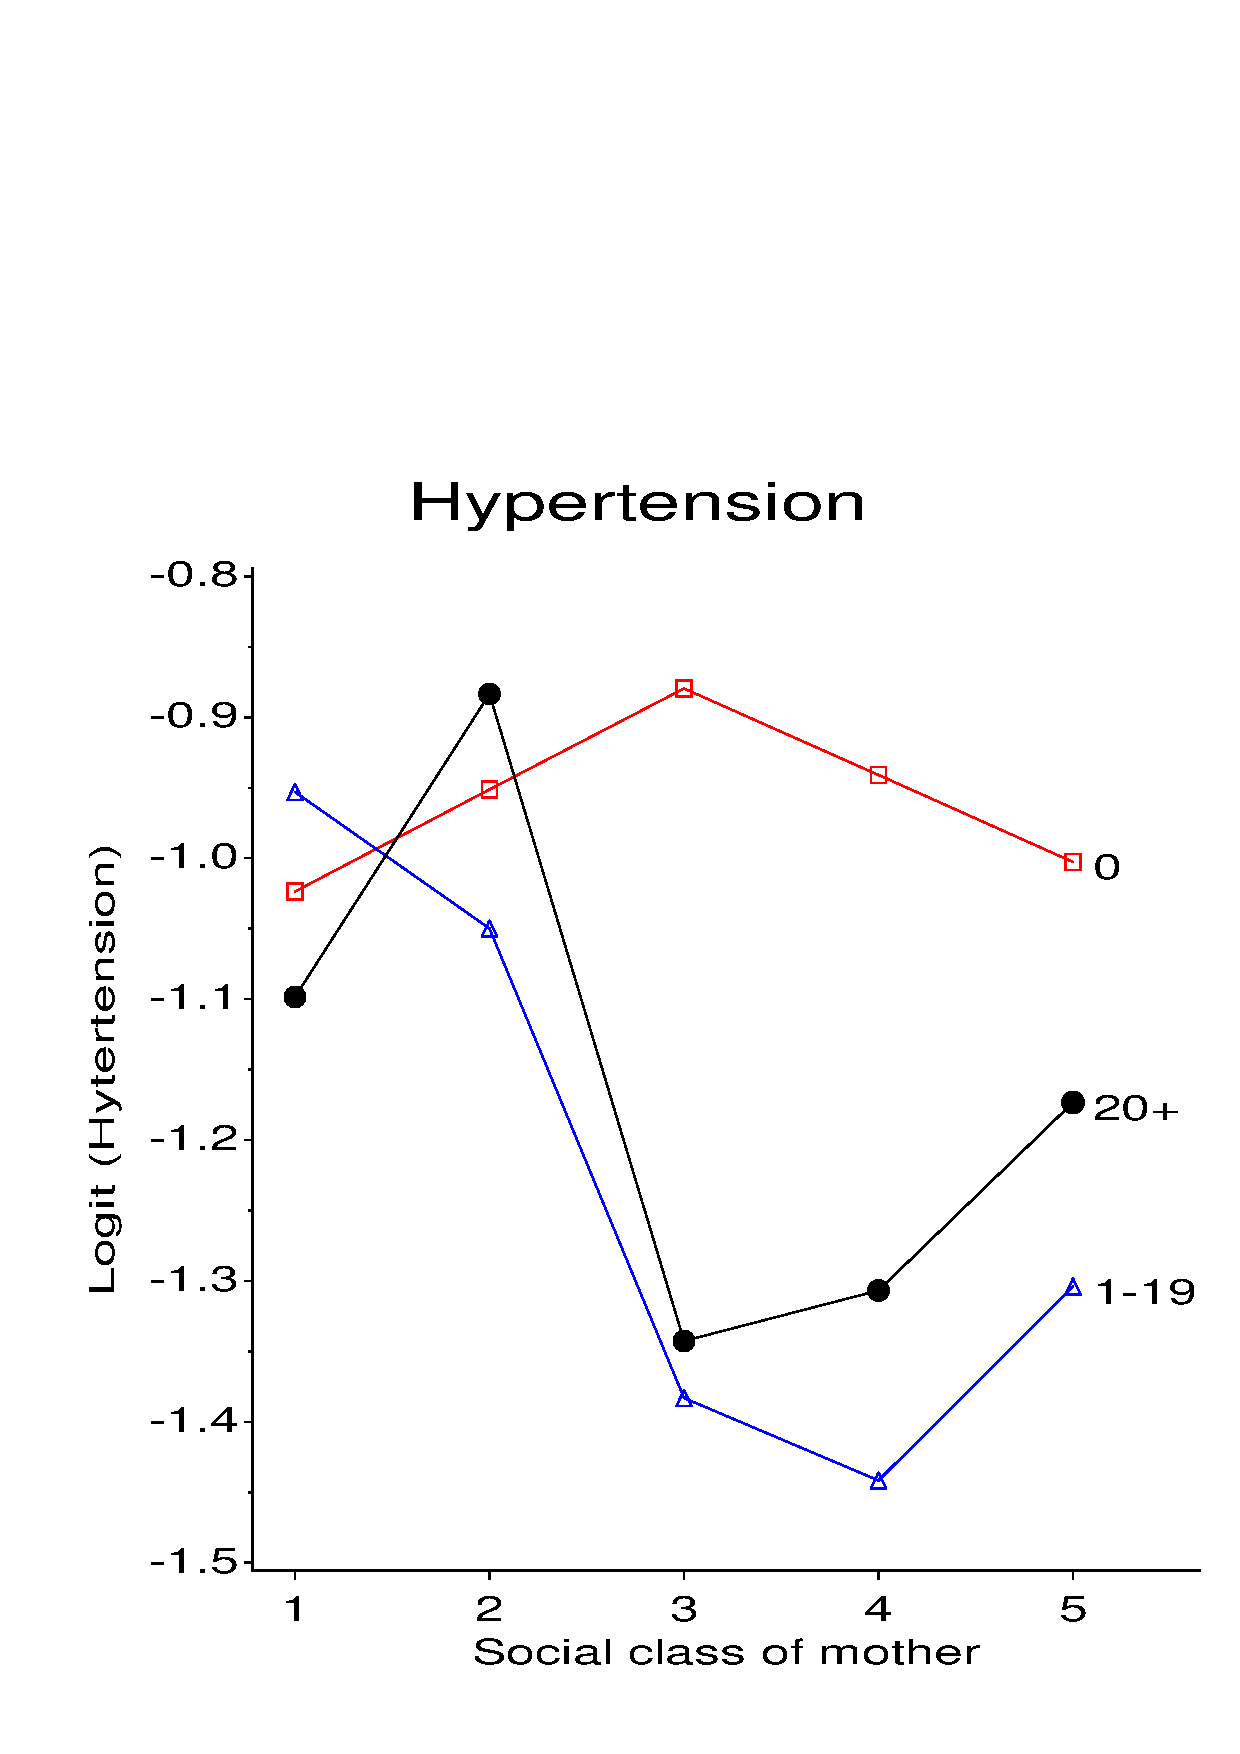
\includegraphics[width=1\linewidth]{tox11}
 \end{minipage}%
 \hfill
 \begin{minipage}[t]{.49\linewidth}
  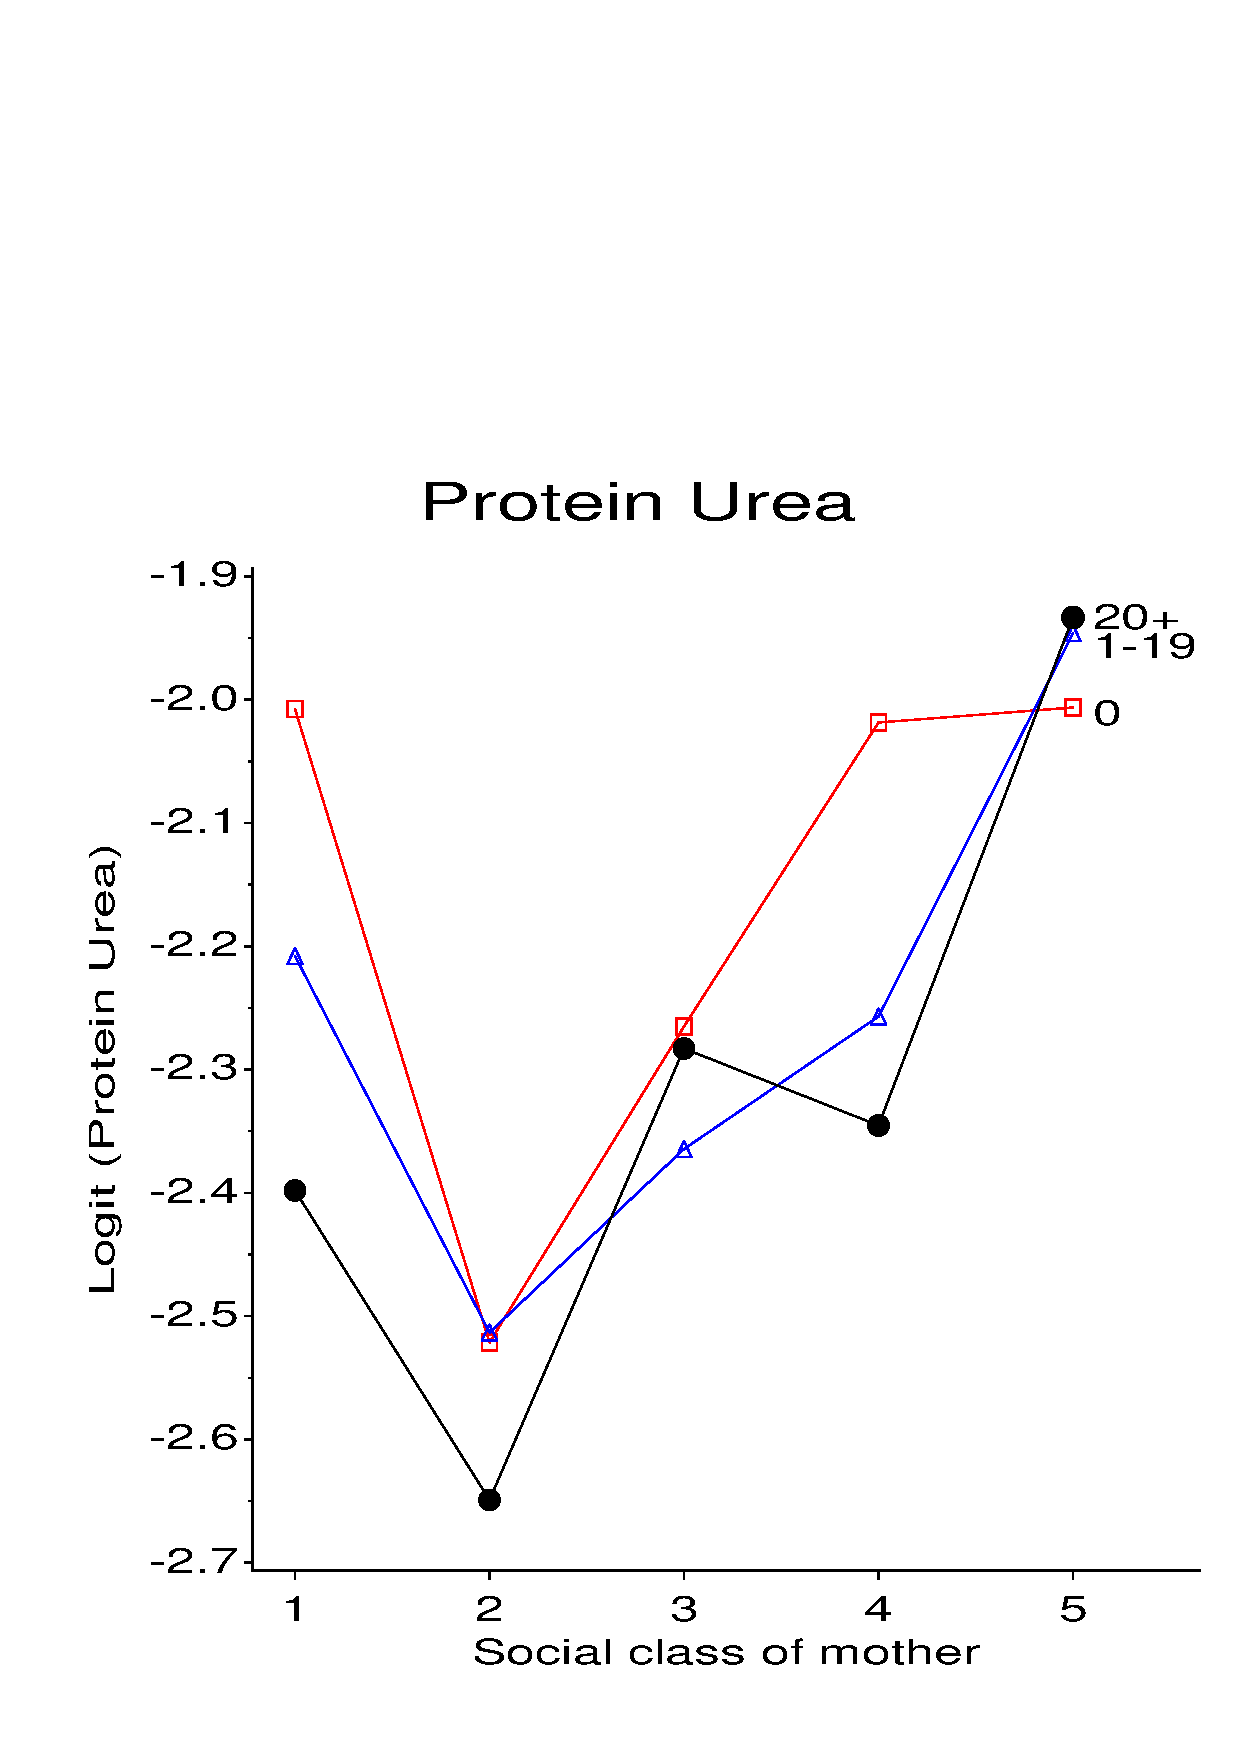
\includegraphics[width=1\linewidth]{tox12}
 \end{minipage}
 \caption{Logits for hypertension and for protein urea, by social class and smoking}\label{fig:tox11}
\end{figure}

From \figref{fig:tox11} it may be seen that the prevalence of these
symptoms has a possibly complex relation to social class and smoking.
However, the mosaic for these predictors in \figref{fig:tox41} has shown
us that several of the class-smoking categories are quite small
(particularly heavy smokers in Class 1)
so the response effects for these classes will be poorly estimated.
Taking this into account,
we suspect that protein urea varies with social class, but not with
smoking, while the prevalence of hypertension may truly vary with neither,
just one, or both of these predictors.

The association between the response symptoms,
shown in \figref{fig:tox13}
is clearer, once we take the variation in sample sizes into account.
Except for the heavy smokers, particularly  in social classes 1 and 2, the log odds ratio
appears to be relatively constant.
%% one figure
\begin{figure}[htb]
  \centering
  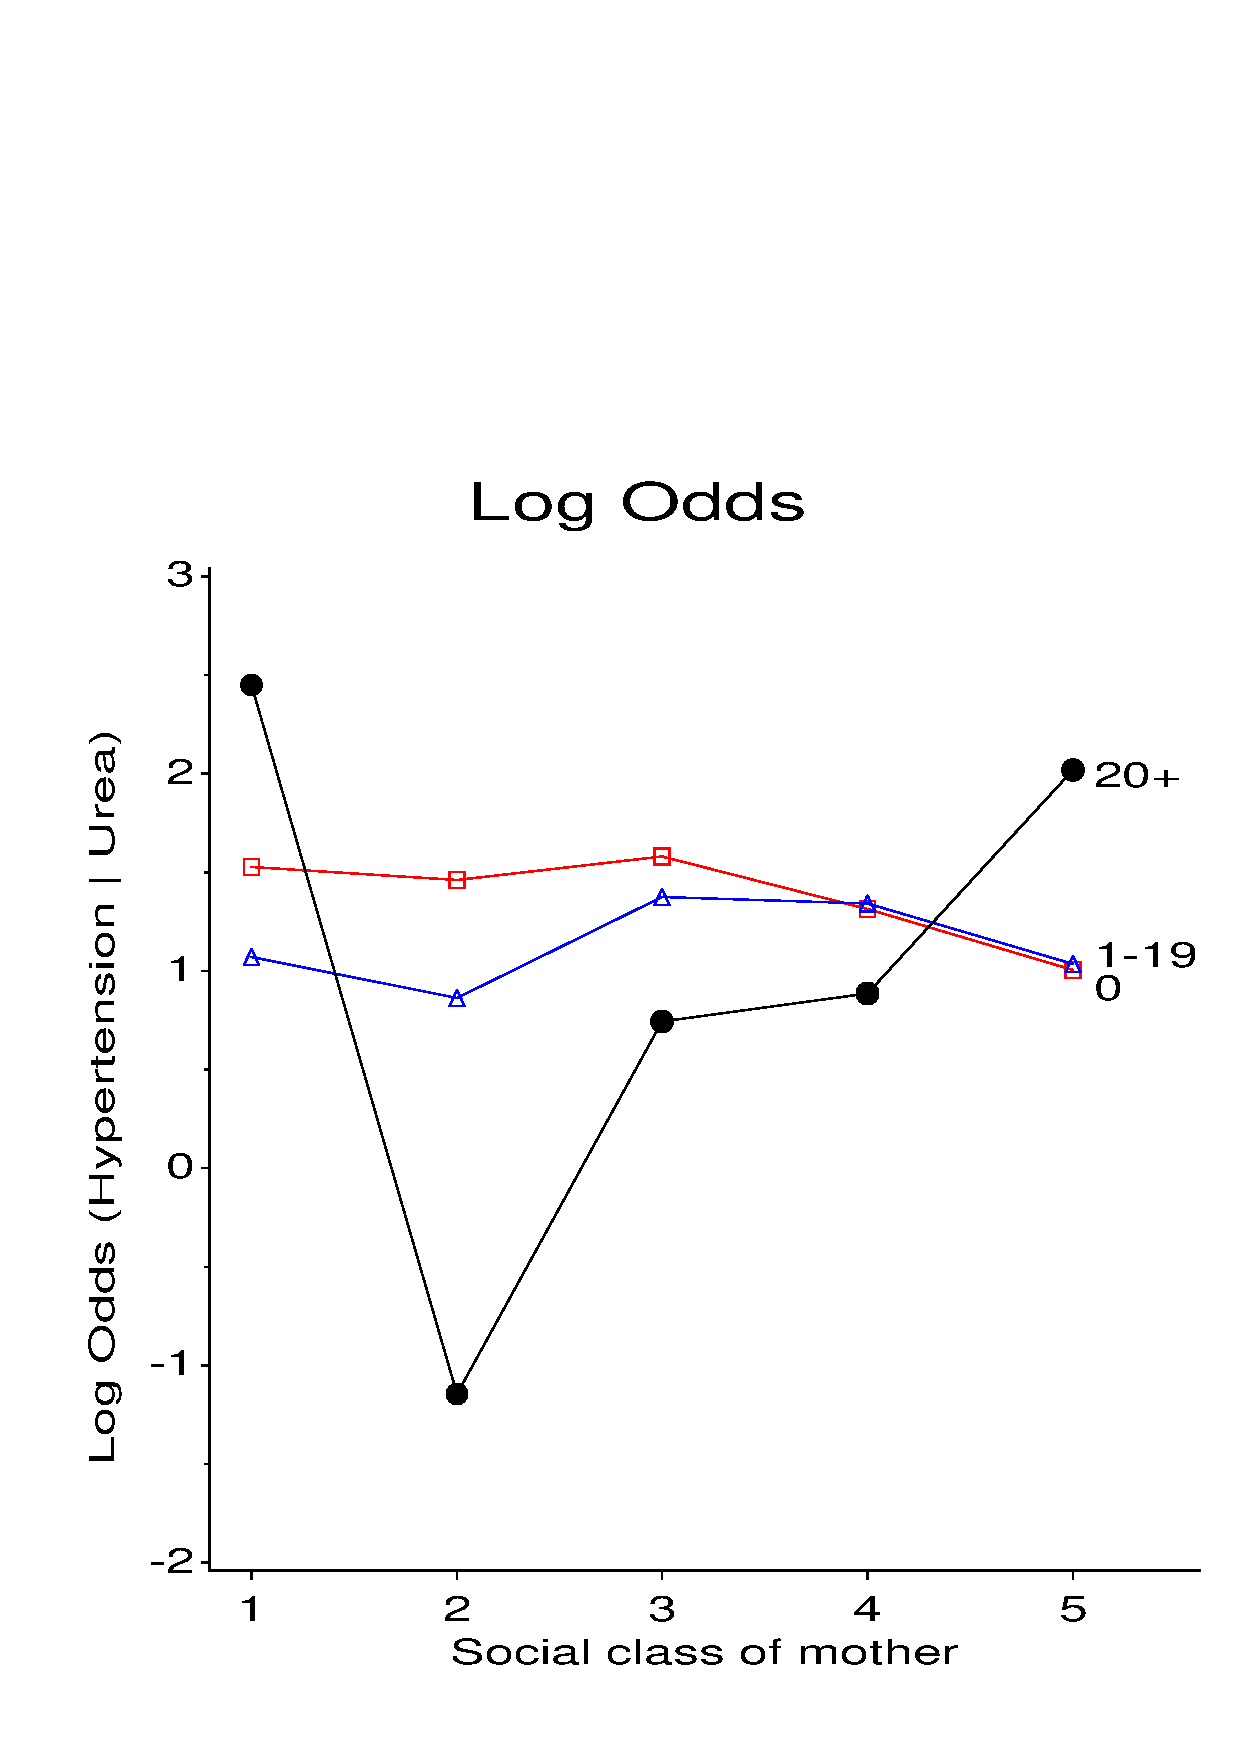
\includegraphics[scale=.4]{tox13}
  \caption{Log odds ratio for hypertension, given protein urea, by social class and smoking}%
  \label{fig:tox13}
\end{figure}

When there are no quantitative predictors, and when the odds ratio is
relatively constant, it is easier to fit ordinary \loglin\ models
than to use the bivariate logit formulation of the previous example.

We fit these models using the \stmt{LOGLIN}{CATMOD} as shown below.
There are two zero cells in \tabref{tab:toxtab}.
In the \loglin\ formulation \PROC{CATMOD} treats these as structural
zeros, so we first replace the zeros with a small positive number.
The minimal model, $[CS] [H] [U]$ fits the marginal association of the
numbers in each Class-Smoking category, but asserts that the responses,
$H$ and $U$ are independent, which we have already seen is contradicted
by the data.  We take $[CS] [HU]$ as the null model (Model 0), asserting no relation
between response and predictor variables.
%% input: /users/faculty/friendly/sasuser/catdata/tox2l.sas
%% last modified: 19-Nov-98  9:23
\begin{listing}
%include catdata(toxaemia);
data toxaemia;
   set toxaemia;
   if count=0 then count=1E-10;

*-- Loglinear models;
proc catmod order=data
            data=toxaemia;
   weight count;
   model hyper*urea*class*smoke =  _response_ /
      ml noiter noresponse noprofile nodesign;
   loglin  class|smoke hyper urea / title='Model -1: CS  H  U';
run;
   loglin  class|smoke hyper|urea / title='Model 0: CS  HU';
run;
   loglin  class|smoke  hyper|urea  hyper|smoke  urea|class /
       title='Model 1: CS  HU  SH  CU';
run;
   loglin  class|smoke|hyper|urea @2 /
       title='Model 2: CS  CH  CU  HU  SH  CU';
run;
   loglin class|smoke|hyper  class|urea  hyper|urea /
       title='Model 3: CSH  CU  HU';
run;
   loglin class|smoke|hyper  class|urea  smoke|urea  hyper|urea /
       title='Model 4: CSH  CU  SU  HU';
run;
   loglin class|smoke|hyper  class|smoke|urea  hyper|urea /
       title='Model 5: CSH  CSU  HU';
run;
\end{listing}


The fit statistics and some model selection criteria for these and other
models are shown in \tabref{tab:toxmod}.
The large residual $G^2$ for Model 0 (179.03 on 42 df) indicates substantial
associations between the responses and explanatory variables.
Model 1 adds the simple dependence of hypertension on smoking ($[SH]$) and that of urea on class ($[CU]$); Model 2 includes all two-way terms.
In Model 3, hypertension is allowed to depend on both class and smoking
jointly ($[CSH]$). In Model 4 an additional dependence of
urea on smoking ($[SU]$) is included, while in Model 5 urea depends on
class and smoking jointly ($[CSU]$).
\begin{table}[htb]
 \caption{Loglinear models fit to toxaemia data}\label{tab:toxmod}
 \begin{center}
 \begin{tabular}{rl rrrrrrr}
  \hline
  Model & Terms         & df & \chisq & $p$-value & \chisq /df & AIC & $R^2$ & Adj. $R^2$ \\ 
  \hline
 -1 & CS H U            & 43 & 672.85 & 0.0000 & 15.65 & 586.85 & . & . \\ 
  0 & CS HU             & 42 & 179.03 & 0.0000 & 4.26 & 95.03 & 0.000 & 0.000 \\ 
  1 & CS HU SH CU       & 36 & 46.12 & 0.1203 & 1.28 & -25.88 & 0.742 & 0.699 \\ 
  2 & CS CH CU HU SH CU & 30 & 40.47 & 0.0960 & 1.35 & -19.53 & 0.774 & 0.684 \\ 
  3 & CSH CU HU         & 24 & 26.00 & 0.3529 & 1.08 & -22.00 & 0.855 & 0.746 \\ 
  4 & CSH CU SU HU      & 22 & 25.84 & 0.2588 & 1.17 & -18.16 & 0.856 & 0.724 \\ 
  5 & CSH CSU HU        & 14 & 22.29 & 0.0729 & 1.59 & -5.71 & 0.875 & 0.626 \\ 
  6 & CSH CSU SHU       & 12 & 15.65 & 0.2079 & 1.30 & -8.35 & 0.913 & 0.694 \\ 
  7 & CSH CSU CHU SHU   & 8 & 12.68 & 0.1233 & 1.59 & -3.32 & 0.929 & 0.628 \\ 
  8 & CSHU              & 0 & 0.00 & . & . & 0.00 & 1.000 & . \\ 
  \hline
 \end{tabular}
 \end{center}
\end{table}


None of these models contain three-way terms involving both $H$ and $U$,
so these models assume that the log odds ratio for hypertension given urea
is constant over the explanatory variables.
Recalling the partial mosaics (\figref{fig:tox42} and \figref{fig:tox43})  Models 6 and 7 add terms
which allow the odds ratio to vary, first with smoking ($[SHU]$), then
with class ($[CHU]$) as well.

How do we choose among these models?  Model 1 is the smallest whose deviance
is non-significant. Models 3 and 4 both have a smaller ratio of \chisq\/df.
For comparing nested models, we can also examine the change in deviance as
terms are added (or dropped).  Thus, going from Model 1 to Model 2
decreases the deviance by 5.65 on 6 df, while the step from Model 2 to Model 3
gives a decrease of 14.47, also on 6 df.  The AIC statistic, balancing
parsimony and goodness-of-fit, has its minimum value for Model 1,
which we adopt here for this example.

Whatever model is chosen, as a final step, it is important to determine what
that model implies about the original research questions.
Because our focus here is on the prevalence of each symptom, and their
association, it is helpful to graph the fitted logits and log odds ratios
implied by the model, as we did in \figref{fig:ash21} and \figref{fig:ash22}.

In \exref{ex:ashford} we fit the bivariate logit model, for which the
response functions were the desired logits and log odds.
Here, where we have fit ordinary \loglin\ models, the fitted logits
can be calculated from the fitted frequencies.
To obtain predicted frequencies under Model 1, we use the option
\pname{PRED=FREQ} on the \stmt{MODEL}{CATMOD}.
%% input: /users/faculty/friendly/sasuser/catdata/tox2.sas
%% last modified: 19-Nov-98 15:21
\begin{listing}
proc catmod order=data data=toxaemia;
   weight count;
   response  / out=predict;
   model hyper*urea*class*smoke =  _response_ / pred=freq
      ml noiter noresponse noprofile nodesign;
   loglin  class|smoke hyper|urea hyper|smoke urea|class /
       title='Model 1: CS  HU  SH  CU';
\end{listing}

Then, the observed and fitted frequencies can be extracted from
the \ODS, and rearranged so that logits and log odds
may be calculated.
%% input: /users/faculty/friendly/sasuser/catdata/tox2.sas
%% last modified: 19-Nov-98 15:27
\begin{listing}
data predict;
   set predict;
   where (_type_='FREQ');
   drop _sample_ _number_ _type_;
proc sort data=predict;
   by class smoke hyper urea;

proc transpose data=predict out=fit(drop=_label_) prefix=fit;
   by class smoke;
   var _pred_;
proc transpose data=predict out=obs(drop=_label_) prefix=obs;
   by class smoke;
   var _obs_;

data pred;
   merge fit obs;
   drop _name_;
   array f\{4\} fit1-fit4;   *-- Fitted frequencies;
   array o\{4\} obs1-obs4;   *-- Observed frequencies;
   
   fhyper = log( (f[1] + f[2] + .5) / (f[3] + f[4] + .5) );
   furea =  log( (f[1] + f[3] + .5) / (f[2] + f[4] + .5) );
   fodds=  log( ((f[1]+.5)*(f[4]+.5))/((f[2]+.5)*(f[3]+.5)) );
   
   ohyper = log( (o[1] + o[2] + .5) / (o[3] + o[4] + .5) );
   ourea =  log( (o[1] + o[3] + .5) / (o[2] + o[4] + .5) );
   oodds=  log( ((o[1]+.5)*(o[4]+.5))/((o[2]+.5)*(o[3]+.5)) );
   
   label fhyper = 'Logit (Hytertension)'
      furea =   'Logit (Protein Urea)'
      fodds = 'Log Odds (Hypertension | Urea)';
   format smoke smoke.;
\end{listing}

%% one figure
\begin{figure}[htb]
  \centering
  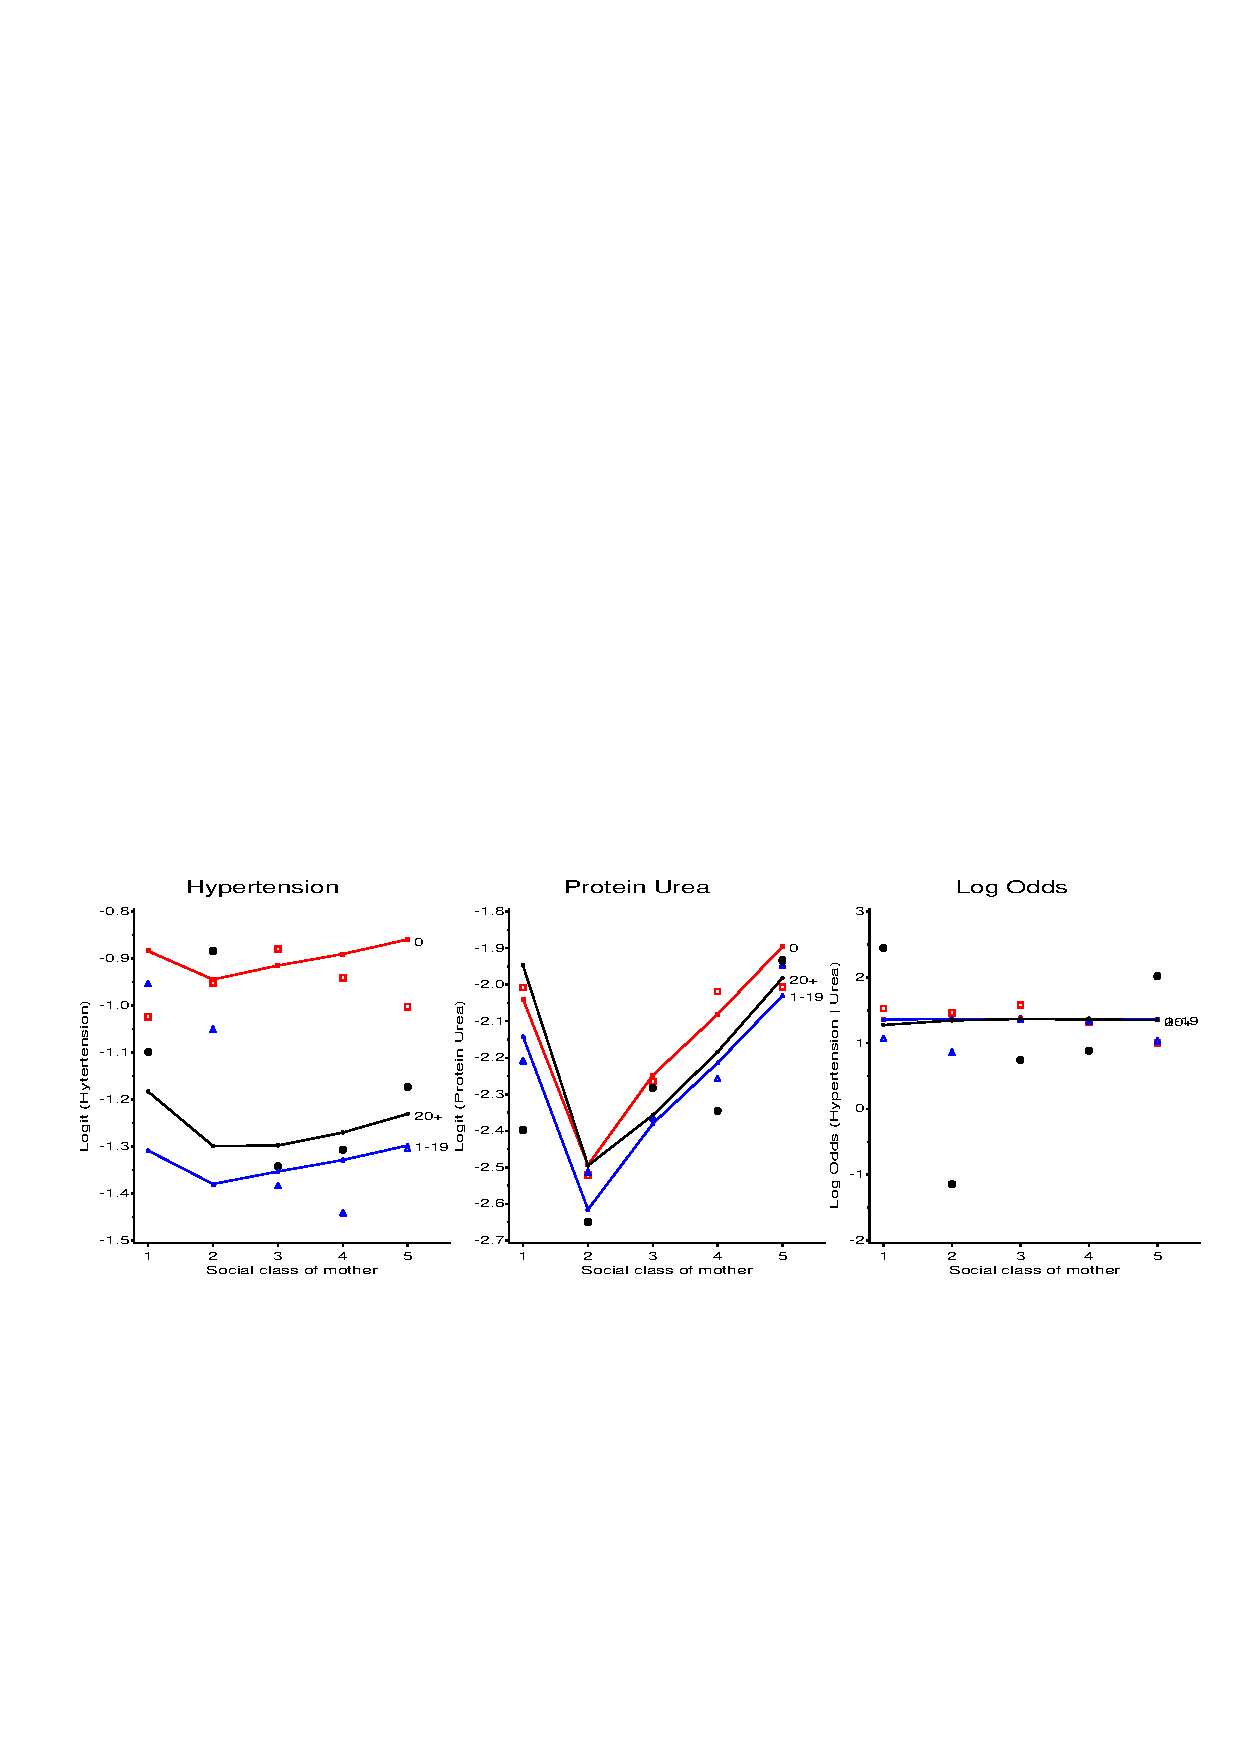
\includegraphics[width=\textwidth,clip]{tox2}
  \caption{Toxaemia data: Observed and fitted logits and log odds ratios for Model 1: $[CS] [HU] [SH] [CU]$}%
  \label{fig:tox2}
\end{figure}
Finally, each measure is plotted separately, showing the fitted values
with curves and the observed values with points.  The statements
below are repeated for urea and for log odds.  The three graphs are
shown in \figref{fig:tox2}.
%% input: /users/faculty/friendly/sasuser/catdata/tox2.sas
%% last modified: 19-Nov-98 15:29
\begin{listing}
%label(data=pred, x=class, y=fhyper, subset=(class=5),
   text=put(smoke, smoke.), pos=6, xoff=.1, out=lab);

%points(data=pred, x=class, y=ohyper, 
   symbol=scan('square triangle dot',smoke),
   color=scan('red blue black', smoke), size=2, out=_pts_);
data lab;
   set lab _pts_;

proc gplot data=pred;
   plot fhyper  * class = smoke / anno=lab nolegend
      vaxis=axis1 haxis=asix2 hm=0 vm=1;
   symbol1 v=square   h=1 i=join c=red;
   symbol2 v=triangle h=1 i=join c=blue;
   symbol3 v=dot      h=1 i=join c=black;
   axis1 label=(a=90) order=(-1.5 to -0.8 by .1);
   axis2 offset=(3,9);
   title 'Hypertension';
\end{listing}

We can see from \figref{fig:tox2} that the fitted log odds ratio is in fact
nearly constant,
while the log odds for hypertension depends mainly on smoking, while
that for protein urea depends mainly on social class.
Yet, the great variability of the observed points around the fitted
curves indicates that these relationships are not well-determined.
Adding error bars showing the standard error around each fitted point
would indicate that the data conforms as closely to the model as
can be expected, given the widely different sample sizes.
However, this would make the plots more complex, and so was omitted
here.
In addition to showing the pattern of the results according to the fitted
model, such graphs also help us to appreciate the model's limitations.
\end{Example}
